
Otra forma de visualizarlo es con un grafo dirigido, en la figura
 \ref{fig:alg02} se aprecia el correspondiente a la cadena
 de entrada del ejemplo anterior (``ABCDEABDEABXGRWACE''), el cual tiene un 
 nodo inicial sin informaci\'on, posteriormente, cada acci\'on realizada por 
 la persona con los dispositivos de entrada (teclado y rat\'on) es un nodo
 \'unico, es decir, a cada acci\'on corresponde un nodo. El cual contiene la 
 tupla de informaci\'on (dispositivo,
 acci\'on y colocaci\'on) de la acci\'on realizada, el tiempo de espera para
 ejecutar dicha acci\'on, y un contador de incidencias para el nodo y la
 referencia a los siguientes.
 
 
\begin{figure}[h!]
\centering
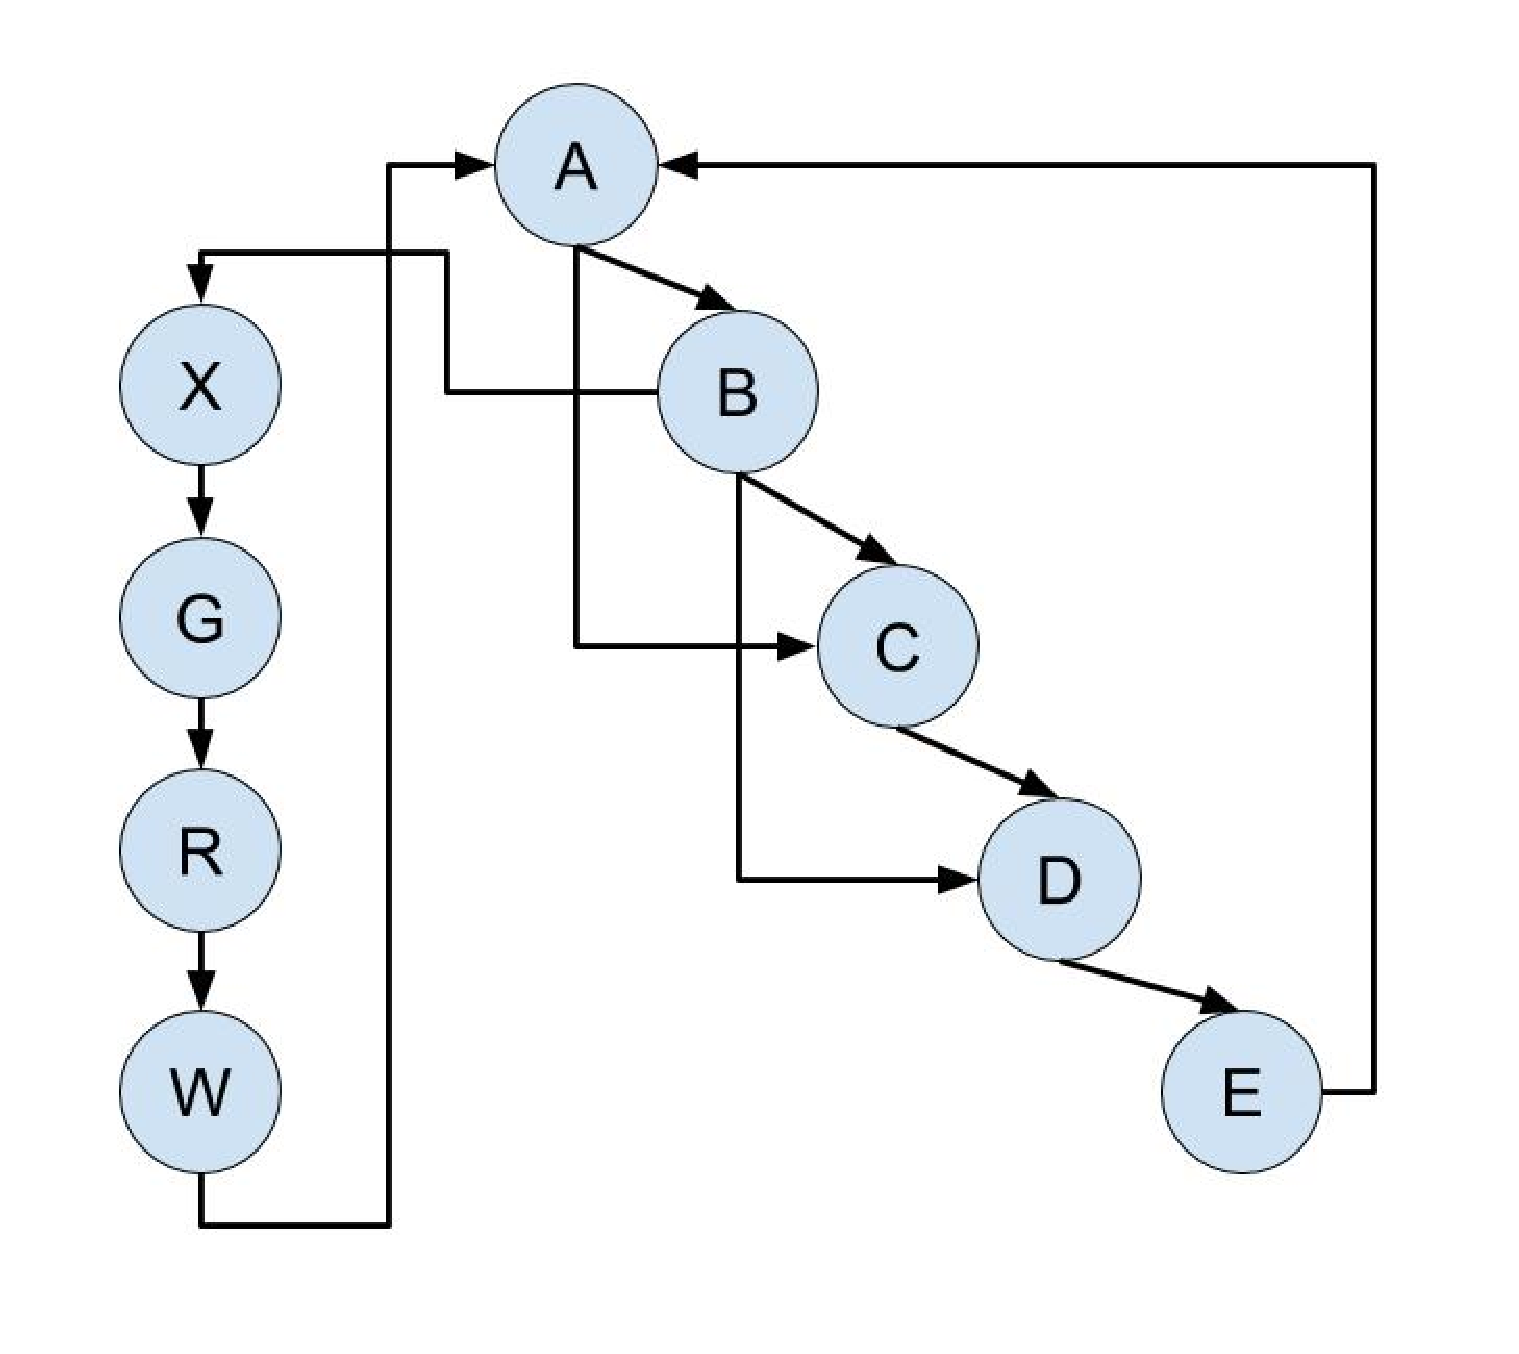
\includegraphics[width=0.5\columnwidth]{chap4/Imagenes/algoritmo2.eps}
\caption{Ejemplo del algoritmo con un grafo dirigido.}
\label{fig:alg02}
\end{figure} 
 
\newpage

En la figura \ref{fig:alg02}, se muestran las mismas cadenas generadas en el 
 ejemplo de la figura \ref{fig:alg01} (``ABCDE'', ``ABDE'', ``ABXGRW'' y 
 ``ACE''), la principal diferencia radica, en la reutilizaci\'on de los nodos, 
 ya que cada vez que se ingrese el car\'acter ``A'', se recurre al nodo 
 generado anteriormente en lugar de generar uno nuevo, esto permite el ahorro 
 de memoria durante la ejecuci\'on y la extracci\'on de la secuencias 
 repetitivas.


Con la anterior definici\'on para los nodos se crea el grafo dirigido,
 siguiendo el algoritmo descrito gr\'aficamente por el diagrama de flujo 
 de la figura \ref{fig:conc01}; cuando se lee una acci\'on se crea el nodo
 (en caso de no existir) y el enlace a est\'e desde el anterior (el nodo
 Inicio, para la primer acci\'on le\'ida), y se sigue as\'i durante la sesi\'on
 del usuario. Cuando una acci\'on se repite, es decir, que ya existe el nodo,
 se busca el nodo ya creado correspondiente a dicha acci\'on, se crea el enlace 
 a este y el contador de incidencias se incrementa por la unidad.

\begin{figure}[]
\centering
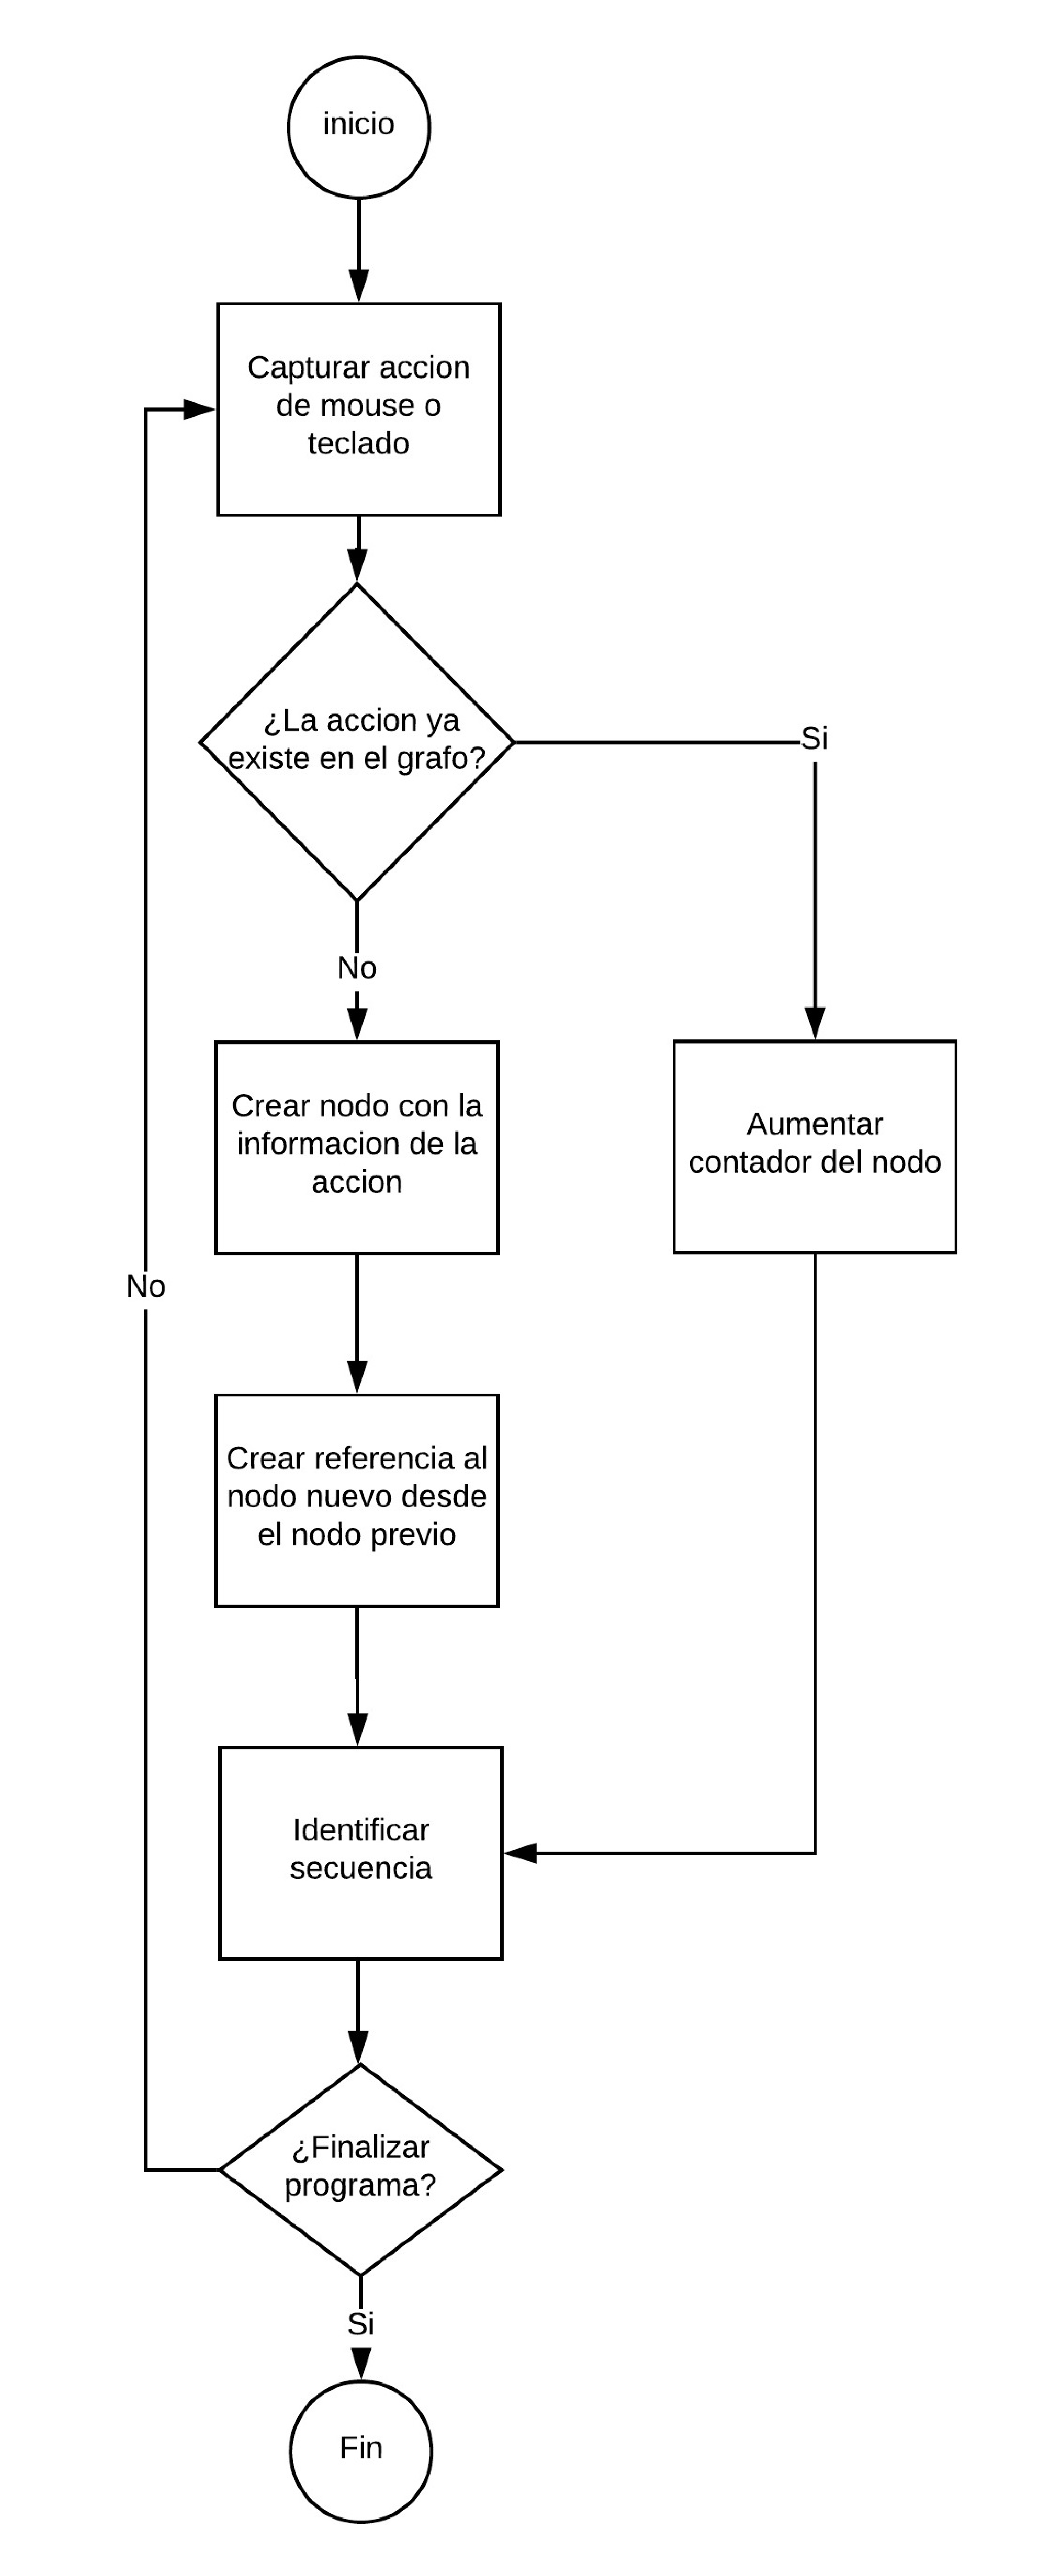
\includegraphics[width=0.5\columnwidth]{chap4/Imagenes/concepto1.eps}
\caption{Diagrama de flujo del algoritmo general.}
\label{fig:conc01}
\end{figure} 

El contador de los nodos es utilizado para conocer la frecuencia de cada 
 acci\'on y definir cu\'ales son relevantes, para este caso de estudio se
 defini\'o emp\'iricamente que la frecuencia del nodo debe ser 70
 incidencias, 
 adem\'as, como se puede ver 
 en la figura \ref{fig:conc02}, para obtener una secuencia de acciones se
 genera una lista con las acciones que se est\'an realizando con el numero 
 de incidencias y de forma similar a la analog\'ia con la m\'aquina
 de Turing (ver figura \ref{fig:alg01}), al momento de encontrar una acci\'on
 que se repite en la secuencia y que esta se haya repetido por lo menos 5
 veces,
 se muestra como sugerencia de secuencia \'util y se reinicia la lista; en 
 caso de ser de utilidad a la persona, este se guardar\'a para su posterior 
 uso con un nombre significativo para la persona, de lo contrario, la 
 secuencia se guarda para evitar que se muestre nuevamente.

\begin{figure}[]
\centering
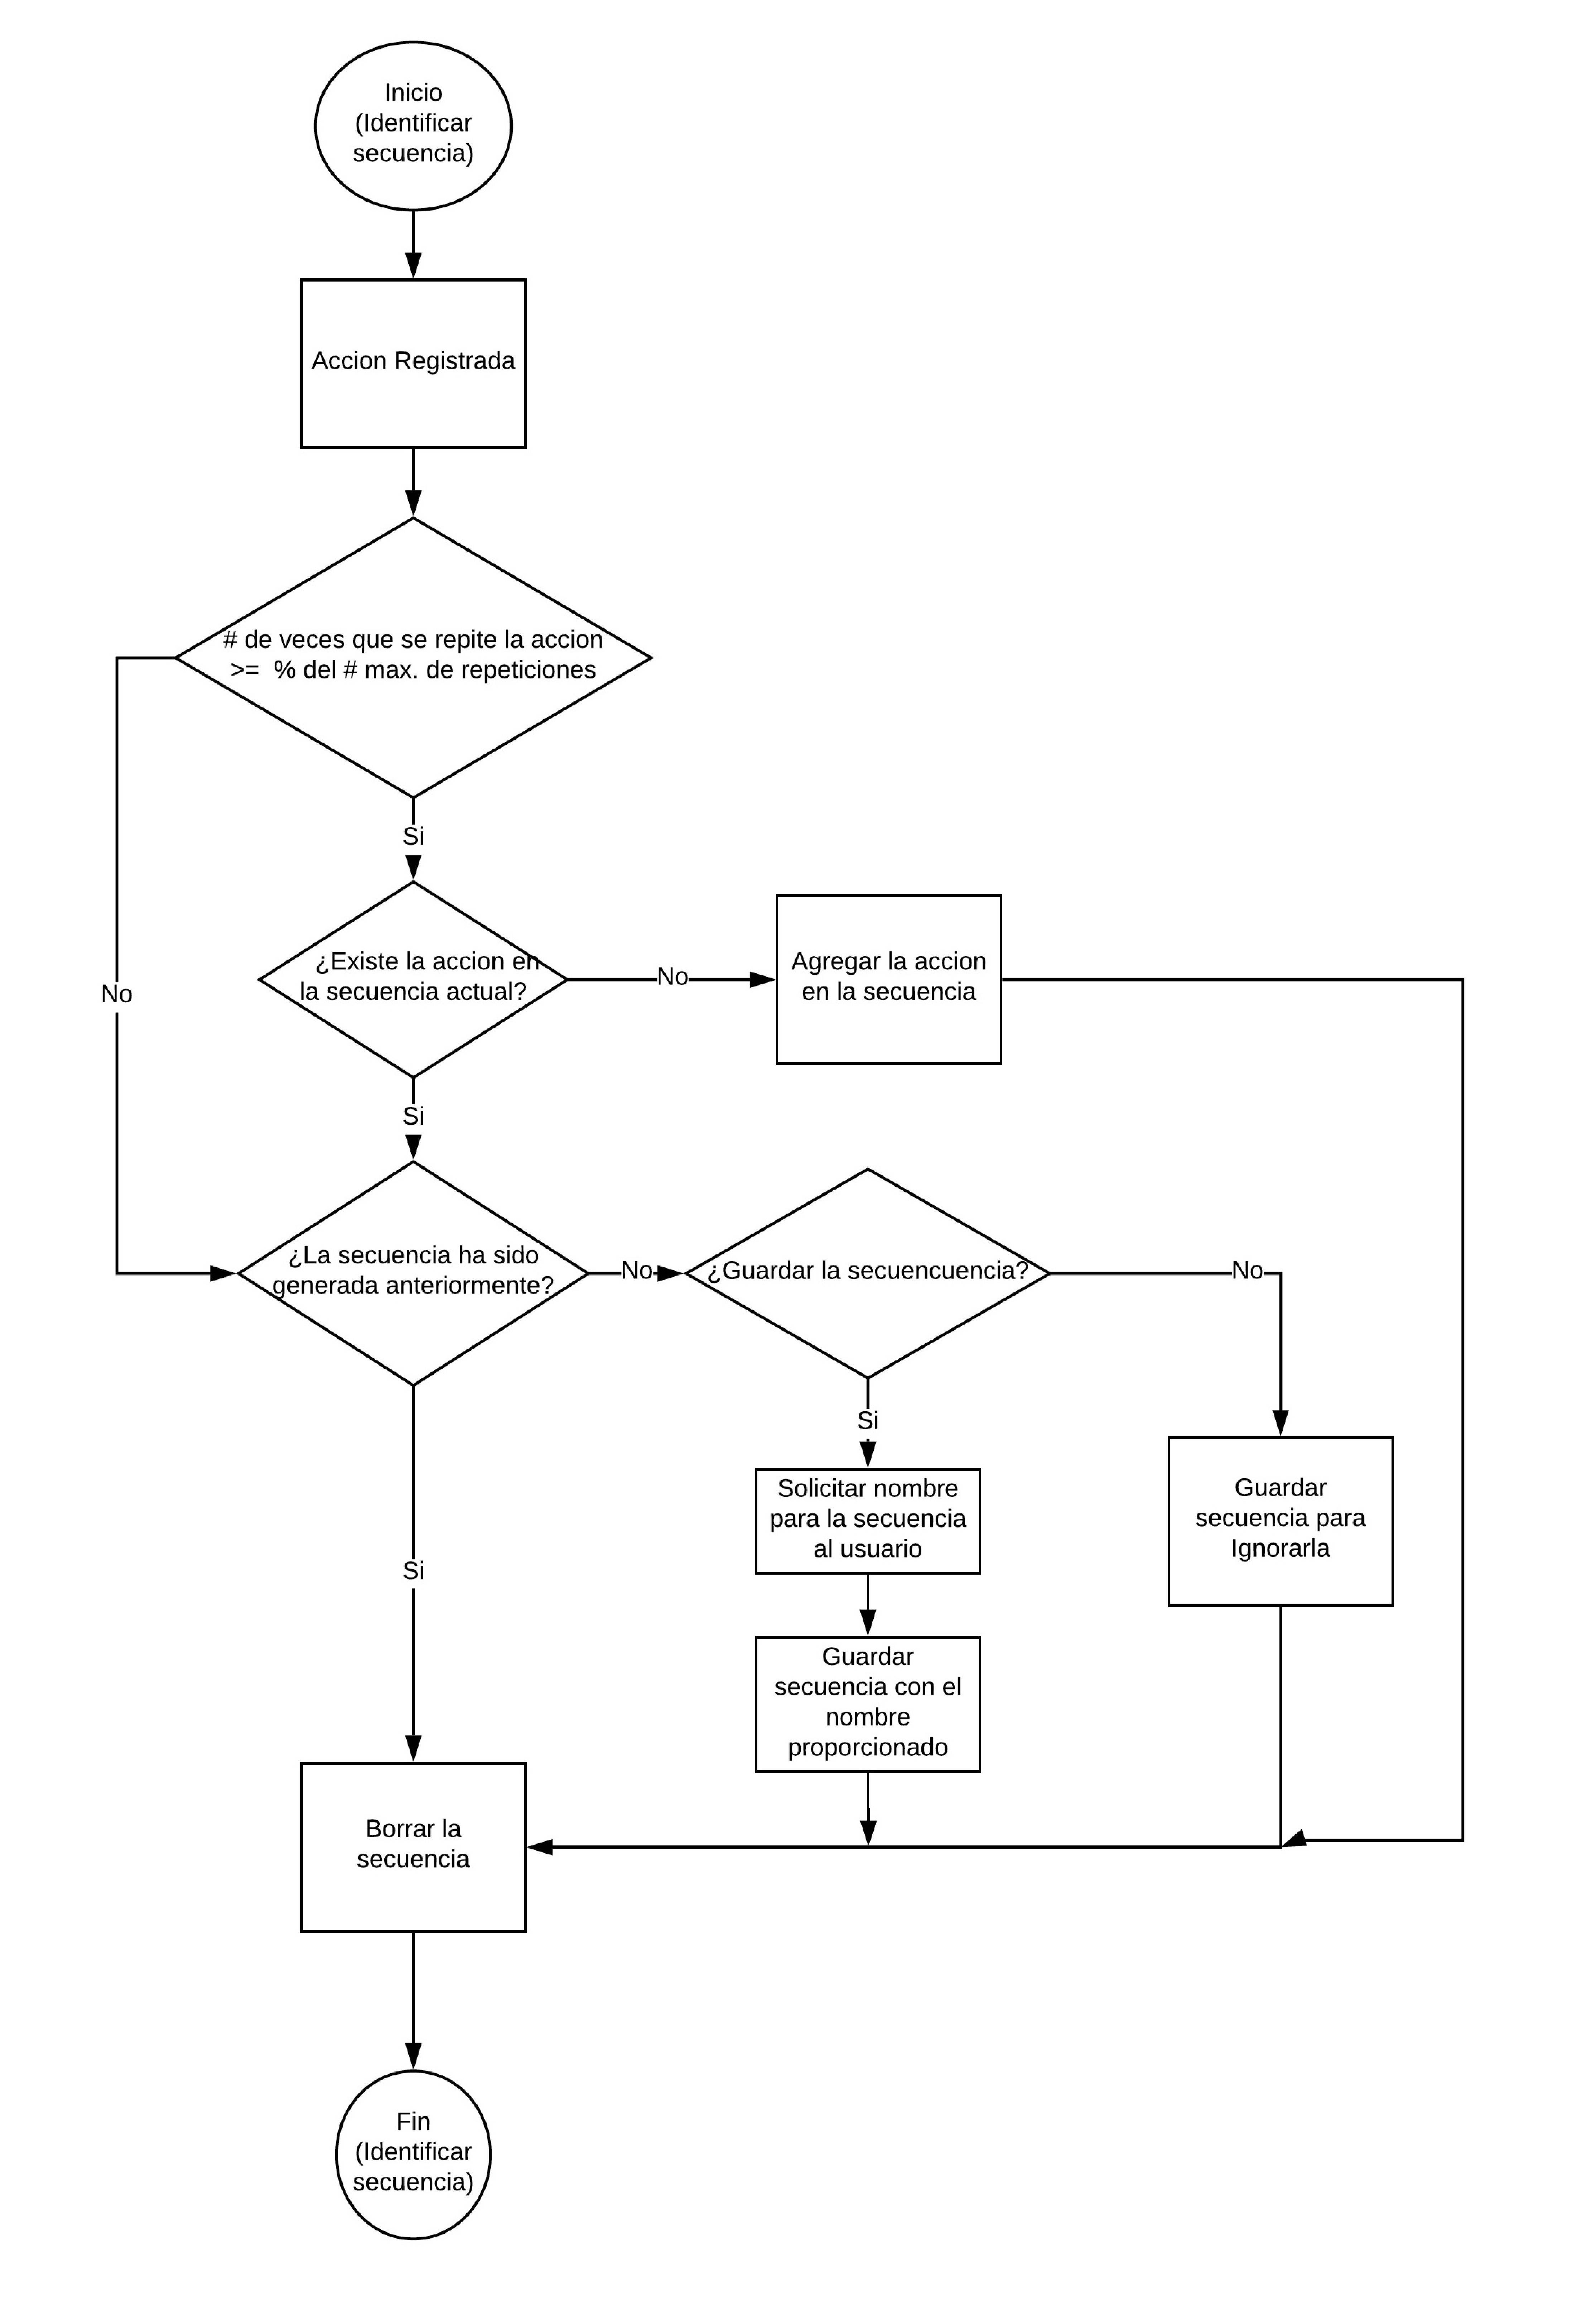
\includegraphics[width=1.0\columnwidth]{chap4/Imagenes/concepto2.eps}
\caption{Diagrama de flujo del bloque ``identificar secuencia'' (ver figura
 \ref{fig:conc01}).}
\label{fig:conc02}
\end{figure} 